\section{Tổng quan bài toán và kiến trúc hệ thống}

\subsection{Bối cảnh và phạm vi kho dữ liệu khoa học arXiv}

Các hệ thống khai phá văn bản khoa học hiện đại thường đối mặt với đánh đổi căn bản giữa khả năng tiếp cận thuận tiện của định dạng PDF và độ trung thực cấu trúc của mã nguồn gốc. Định dạng PDF được thiết kế chủ yếu phục vụ hiển thị trang in, do đó quá trình kết xuất đã làm thất lạc ranh giới phân cấp giữa các mục lớn nhỏ, phá vỡ cấu trúc ký hiệu toán học thành tọa độ phông chữ rời rạc, làm nhiễu thứ tự đọc ở bố cục nhiều cột và cắt đứt liên kết tường minh giữa câu văn với khóa trích dẫn thư mục. Trái lại, khoảng $97\%$ bài nộp trên kho lưu trữ học thuật arXiv cung cấp trực tiếp gói mã nguồn LaTeX nguyên bản~\cite{ginev2024}, cho phép bảo toàn đầy đủ cây cấu trúc tài liệu, công thức toán học chuẩn tắc, mục lục BibTeX và bối cảnh trích dẫn nội tuyến. Không dừng lại ở bản công bố cuối cùng, việc thu hoạch và phân tích đồng thời toàn bộ chuỗi lịch sử phiên bản của từng bài báo (từ phiên bản nộp đầu tiên $v_1$ đến tối đa $v_{13}$ trong tập dữ liệu khảo sát) mở ra khả năng theo dõi tiến hóa nội dung khoa học, đồng thời đặt ra bài toán khử trùng lặp cấu trúc ở quy mô hàng chục triệu nút. Khi kết hợp nguồn toàn văn giàu cấu trúc này với đồ thị trích dẫn liên kết từ nền tảng dữ liệu mở Semantic Scholar~\cite{kinney2023}, hệ thống hình thành nền tảng dữ liệu định lượng phục vụ trực tiếp bài toán học máy đối sánh tài liệu tham khảo theo chuẩn yêu cầu của đồ án môn Nhập môn Khoa học Dữ liệu~\cite{hcmus_intro_ds}.

Phạm vi dữ liệu của nhóm ChickenDev bao phủ năm dải mã định danh arXiv không giao nhau trong giai đoạn từ tháng $09/2024$ đến tháng $07/2025$, tạo thành kho dữ liệu chính thức gồm chính xác $25{,}000$ bài báo khoa học chia đều $5{,}000$ bài cho mỗi thành viên. Trong số này, ba dải nằm trọn trong một tháng dương lịch ($09/2024$, $01/2025$ và $03/2025$) nên chỉ cần kiểm tra đúng $5{,}000$ mã ứng viên mỗi dải, còn hai dải bắc ngang ranh giới chuyển tháng ($04\text{--}05/2025$ và $06\text{--}07/2025$) buộc hệ thống phải dò quét tuần tự lần lượt $83{,}142$ và $80{,}870$ mã ứng viên nhằm bảo đảm không bỏ sót bài báo hợp lệ nào gần ngưỡng kết thúc tháng vốn không được công bố trước. Tính tổng thể trên cả năm dải, quy trình dò tìm đã kiểm định $179{,}012$ mã ứng viên để xác nhận $25{,}000$ bài báo chính thức với $40{,}896$ phiên bản khai báo (trung bình $1.636$ phiên bản mỗi bài) và thu hoạch được $466{,}763$ liên kết tài liệu tham khảo có định danh arXiv. Ở tầng phân tích cấu trúc, $22{,}961$ bài báo ($91.84\%$) trải rộng trên $37{,}967$ phiên bản có mã nguồn TeX hợp lệ đã được bóc tách và nén khử trùng lặp xuống còn $11{,}098{,}189$ phần tử nội dung duy nhất nối nhau bởi $16{,}185{,}255$ cạnh quan hệ phân cấp, song hành với $975{,}674$ mục lục BibTeX hợp nhất. Từ toàn bộ kho dữ liệu chuẩn hóa này, một tập mẫu phân tầng gồm $2{,}525$ bài báo ($25$ bài gán nhãn thủ công và $2{,}500$ bài gán nhãn tự động) chứa $101{,}441$ mục BibTeX được trích xuất làm dữ liệu đầu vào cho bài toán xếp hạng và đối sánh tham khảo ở giai đoạn cuối, như tổng hợp chi tiết trong Bảng~\ref{tab:corpus_ranges}.

\begin{table}[htbp]
    \centering
    \scriptsize
    \setlength{\tabcolsep}{3.5pt}
    \renewcommand{\arraystretch}{1.24}
    \begin{tabularx}{\textwidth}{@{}l X r r r r r r@{}}
        \toprule
        \textbf{Thành viên} & \textbf{Dải mã arXiv (Giai đoạn)} &
        \shortstack[r]{\textbf{Ứng}\\\textbf{viên}} &
        \shortstack[r]{\textbf{Phiên}\\\textbf{bản}} &
        \shortstack[r]{\textbf{Trích dẫn}\\\textbf{arXiv}} &
        \shortstack[r]{\textbf{Bài}\\\textbf{M2}} &
        \shortstack[r]{\textbf{Phần tử}\\\textbf{duy nhất}} &
        \shortstack[r]{\textbf{Mục}\\\textbf{BibTeX}} \\
        \midrule
        Trịnh Huỳnh Nhi & 2409.03594 -- 2409.08593 (09/2024) & 5,000 & 8,268 & 91,161 & 4,578 & 2,167,101 & 195,076 \\
        Ngô Mẫn Nhi & 2501.12642 -- 2501.17641 (01/2025) & 5,000 & 8,251 & 78,635 & 4,544 & 2,221,136 & 195,360 \\
        Huỳnh Huy Hoàng & 2503.06914 -- 2503.11913 (03/2025) & 5,000 & 8,384 & 108,616 & 4,664 & 2,198,596 & 203,414 \\
        Phạm Minh Trọng & 2504.17523 -- 2505.00665 (04--05/2025) & 83,142 & 8,060 & 91,814 & 4,585 & 2,288,312 & 194,577 \\
        Nguyễn Phúc Khang & 2506.20788 -- 2507.01658 (06--07/2025) & 80,870 & 7,933 & 96,537 & 4,590 & 2,223,044 & 187,247 \\
        \midrule
        \textbf{Tổng toàn nhóm} & \textbf{5 dải (25,000 bài báo chính thức)} & \textbf{179,012} & \textbf{40,896} & \textbf{466,763} & \textbf{22,961} & \textbf{11,098,189} & \textbf{975,674} \\
        \bottomrule
    \end{tabularx}
    \caption[Phạm vi năm dải dữ liệu arXiv và quy mô tích lũy qua ba giai đoạn]{Phạm vi năm dải dữ liệu arXiv được giao (mỗi dải chính xác 5,000 bài báo) và quy mô kho dữ liệu tích lũy qua ba giai đoạn xử lý. Tỷ lệ phân tích thành công toàn nhóm ở Giai đoạn 2 đạt 91.84\% số bài báo (37,967 trên 40,896 phiên bản) với 16,185,255 cạnh phân cấp; Giai đoạn 3 đánh giá trên tập mẫu 2,525 bài báo gồm 101,441 mục BibTeX.}
    \label{tab:corpus_ranges}
\end{table}

\subsection{Kiến trúc tổng thể ba giai đoạn và mô hình dữ liệu chuẩn hóa}

Thay vì xây dựng một quy trình đơn khối nơi mọi sự cố mạng hoặc tinh chỉnh cú pháp đều buộc phải chạy lại từ đầu, hệ thống được thiết kế theo kiến trúc đường ống ba giai đoạn tách biệt rạch ròi qua các hợp đồng dữ liệu bất biến, minh họa trong Hình~\ref{fig:e2e_architecture}. Giai đoạn 1 phụ trách thu thập dữ liệu đa nguồn từ ba dịch vụ chuyên biệt của arXiv (cổng tìm kiếm Atom, giao thức thu hoạch siêu dữ liệu OAI-PMH và máy chủ gương xuất mã nguồn) kết hợp với đồ thị tri thức học thuật Semantic Scholar, tích hợp lọc nhị phân ngay tại thời điểm giải nén và cơ chế xuất bản giao dịch hai pha có lưu điểm phục hồi. Giai đoạn 2 tiếp nhận các gói mã nguồn đã lọc sạch để gom tệp theo đường biên dịch thực tế, chuẩn hóa văn bản và ký hiệu toán học, tách câu bằng bộ tách tất định, dựng cây cấu trúc phân cấp, hợp nhất thư mục BibTeX và khử trùng lặp phần tử nội dung xuyên phiên bản. Giai đoạn 3 đọc trực tiếp các bảng cột đã chuẩn hóa từ hai giai đoạn trước để thực hiện chọn mẫu phân tầng, xây dựng bộ nhãn chuẩn kết hợp gán nhãn thủ công và luật tự động, trích xuất hai mươi bốn đặc trưng so khớp theo năm nhóm, tiến hành kiểm định chéo theo nhóm bài báo nhằm chọn mô hình tối ưu và xuất bản kết quả dự đoán cuối cùng. Cơ chế cách ly hợp đồng chặt chẽ bảo đảm mọi giai đoạn hạ nguồn chỉ phụ thuộc vào lược đồ bảng đã được kiểm định toàn vẹn tham chiếu của giai đoạn thượng nguồn, nhờ đó việc điều chỉnh quy tắc tách câu hay tái huấn luyện mô hình xếp hạng không bao giờ kích hoạt lại lưu lượng truy vấn mạng tốn kém tới máy chủ bên ngoài.

\begin{figure}[htbp]
    \centering
    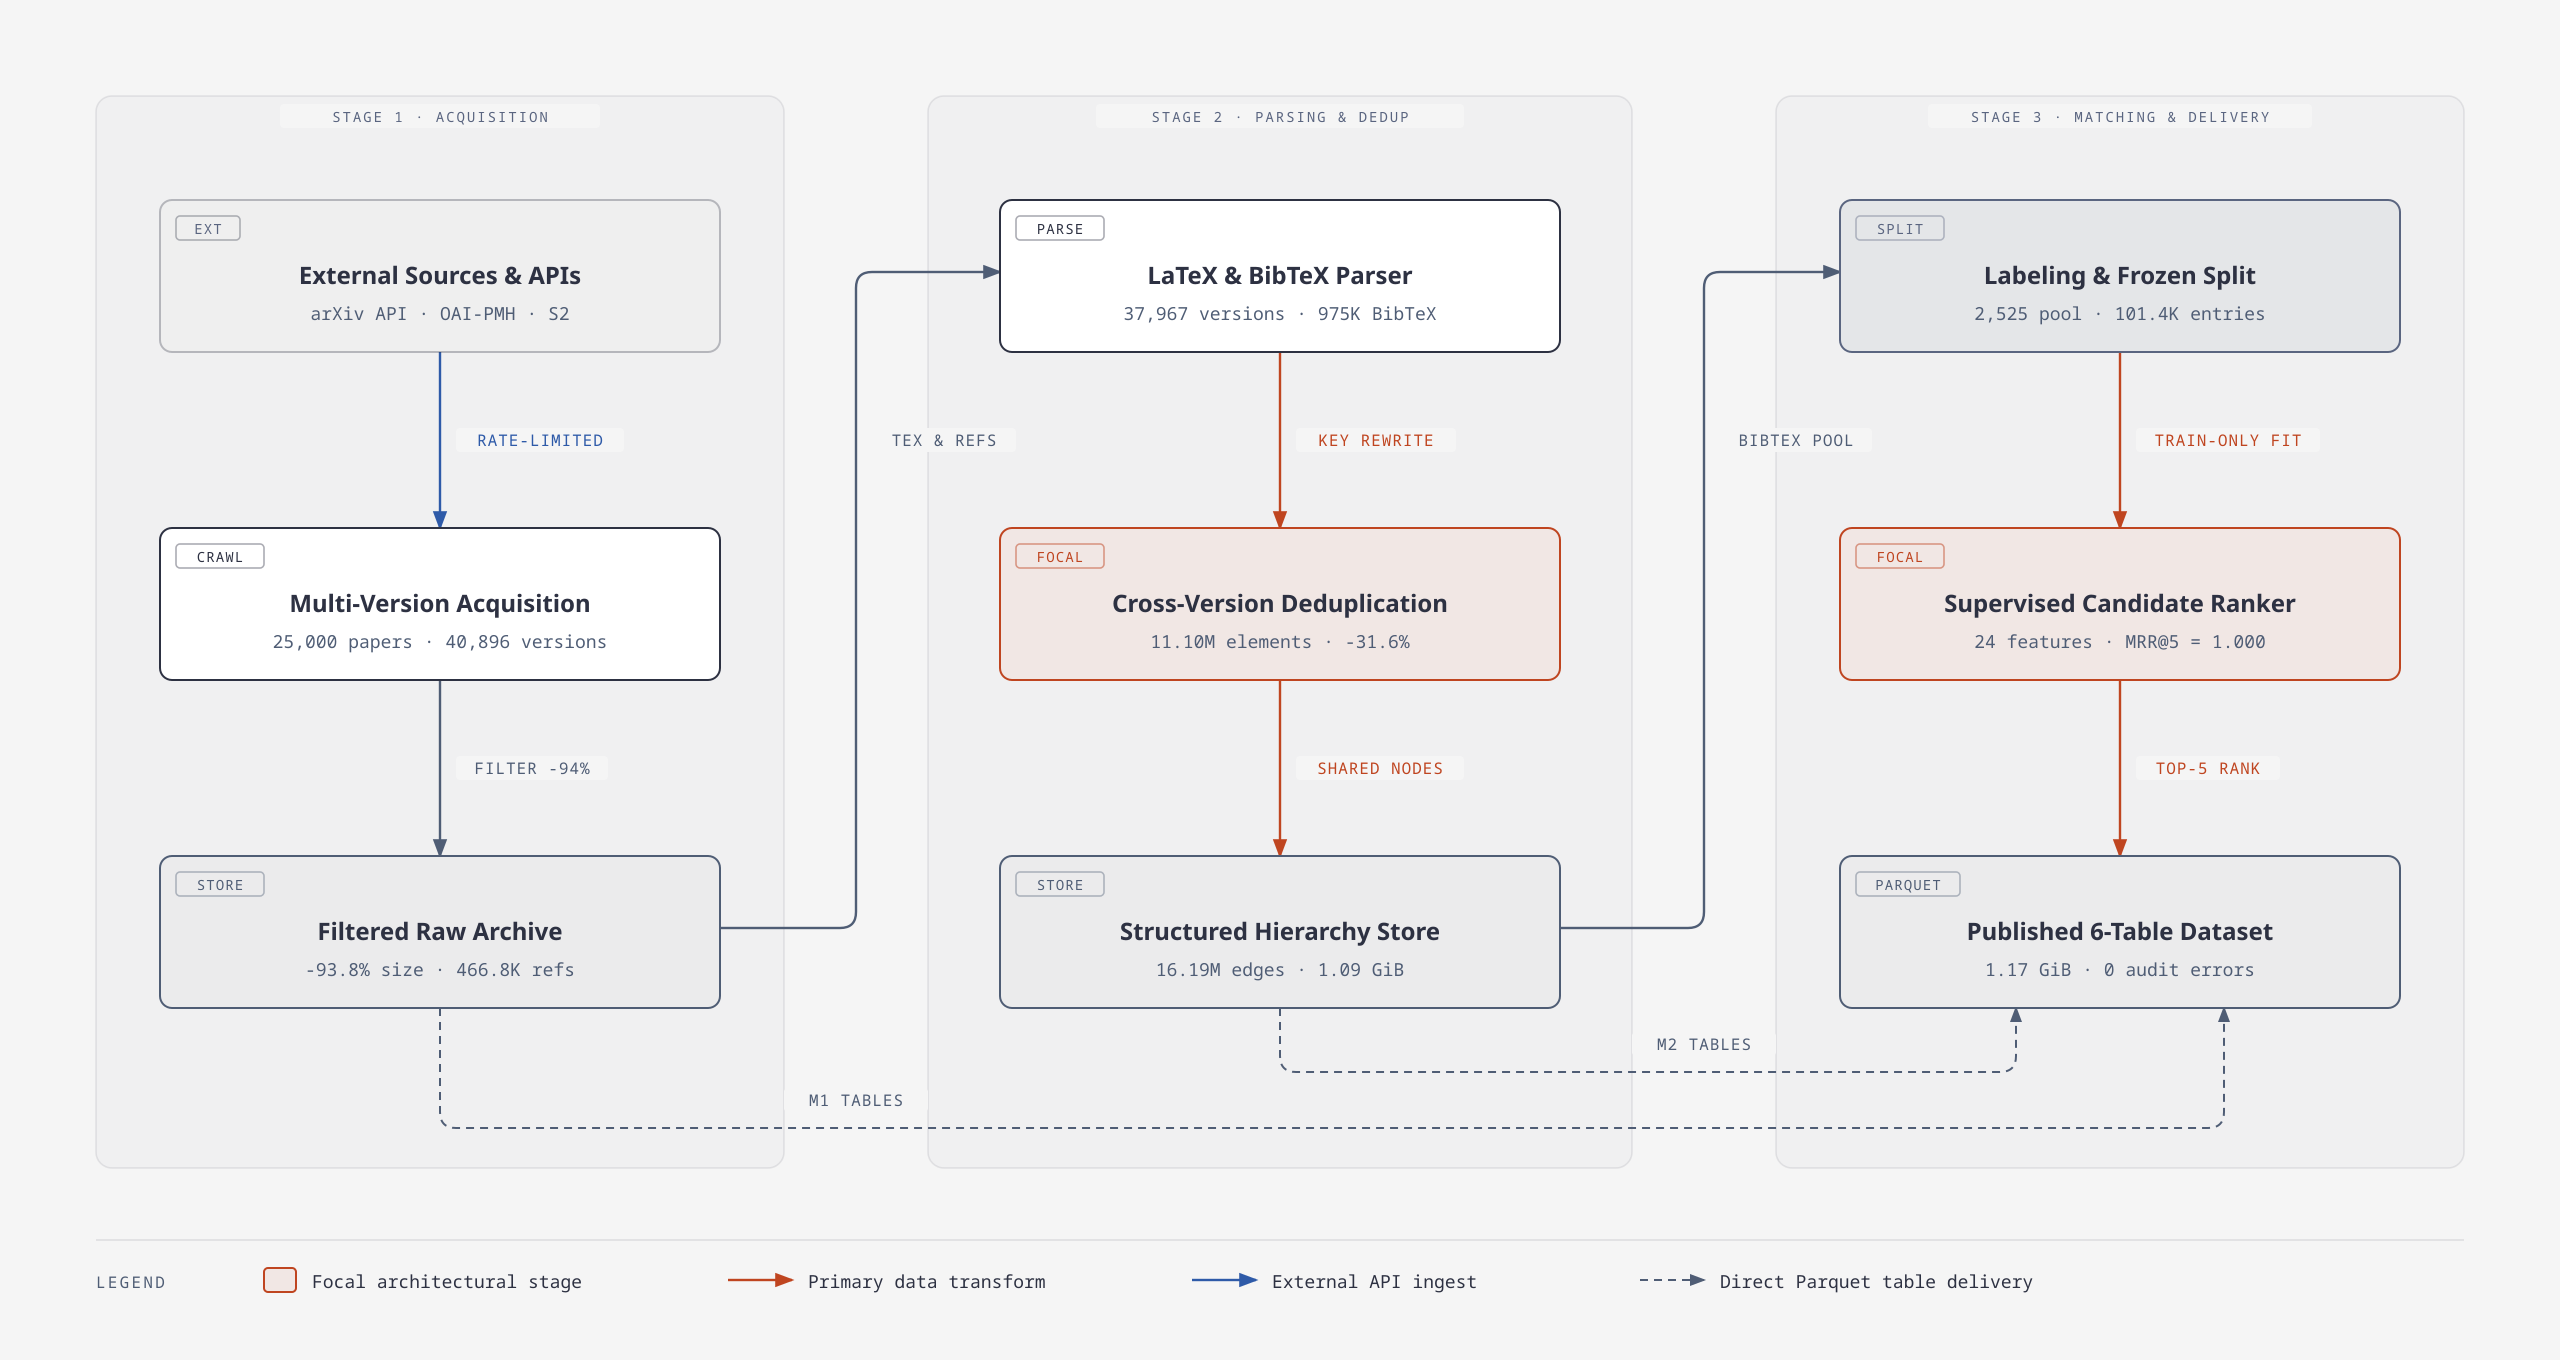
\includegraphics[width=\linewidth]{images/e2e_architecture.png}
    \caption[Kiến trúc tổng thể ba giai đoạn của hệ thống xử lý kho bài báo arXiv]{Kiến trúc tổng thể ba giai đoạn của hệ thống khai thác, phân tích phân cấp và đối sánh tài liệu tham khảo trên kho $25{,}000$ bài báo arXiv, nhấn mạnh ranh giới cách ly hợp đồng dữ liệu, cơ chế vận hành thuần CPU và sáu bảng xuất bản định dạng cột Parquet.}
    \label{fig:e2e_architecture}
\end{figure}

Hai nguyên tắc kỹ thuật xuyên suốt toàn bộ kiến trúc là tính tuân thủ học thuật tuyệt đối về không sử dụng tri thức tiền huấn luyện bên ngoài và khả năng tái lập hoàn toàn trên phần cứng CPU phổ thông~\cite{hcmus_intro_ds}. Hệ thống không gọi bất kỳ mô hình ngôn ngữ lớn, vectơ nhúng ngữ nghĩa tiền huấn luyện hay dịch vụ suy luận ngoài nào trong các khâu chuẩn hóa văn bản, gán nhãn, rút trích đặc trưng và huấn luyện mô hình đối sánh; toàn bộ từ điển n-gram ký tự TF-IDF, hệ số chuẩn hóa và tham số mô hình học có giám sát đều được ước lượng hoàn toàn bên trong tập huấn luyện với hạt giống ngẫu nhiên cố định. Về mặt hạ tầng tính toán, các công đoạn nặng về mạng và nhập xuất được thiết kế chịu lỗi trên máy ảo đám mây Google Colab có tài nguyên khiêm tốn ($2$ vCPU và khoảng $12.68\text{ GiB}$ RAM), trong khi toàn bộ lượt huấn luyện, kiểm định chéo năm phần và suy luận Giai đoạn 3 cho cả năm thành viên chỉ tiêu tốn $12.88\text{ phút}$ trên $2$ luồng CPU với đỉnh bộ nhớ $2{,}393.5\text{ MB}$. Ở tầng lưu trữ phát hành, thay vì duy trì hàng trăm nghìn tệp văn bản rời rạc gây nghẽn hệ thống tệp, toàn bộ kết quả ba giai đoạn được hợp nhất thành sáu bảng dữ liệu phân mảnh theo định dạng lưu trữ cột Apache Parquet~\cite{apache_parquet}. Cơ chế nén theo cột kết hợp mã hóa từ điển giúp toàn bộ kho dữ liệu $25{,}000$ bài báo đa phiên bản (bao gồm hơn $11$ triệu phần tử nội dung và hơn $16$ triệu cạnh phân cấp) chỉ chiếm đúng $1{,}199.45\text{ MiB}$ ($1.171\text{ GiB}$), đồng thời hỗ trợ truy vấn chọn lọc cột trực tiếp mà không cần giải nén toàn bộ bảng vào bộ nhớ chính.

\begin{figure}[htbp]
    \centering
    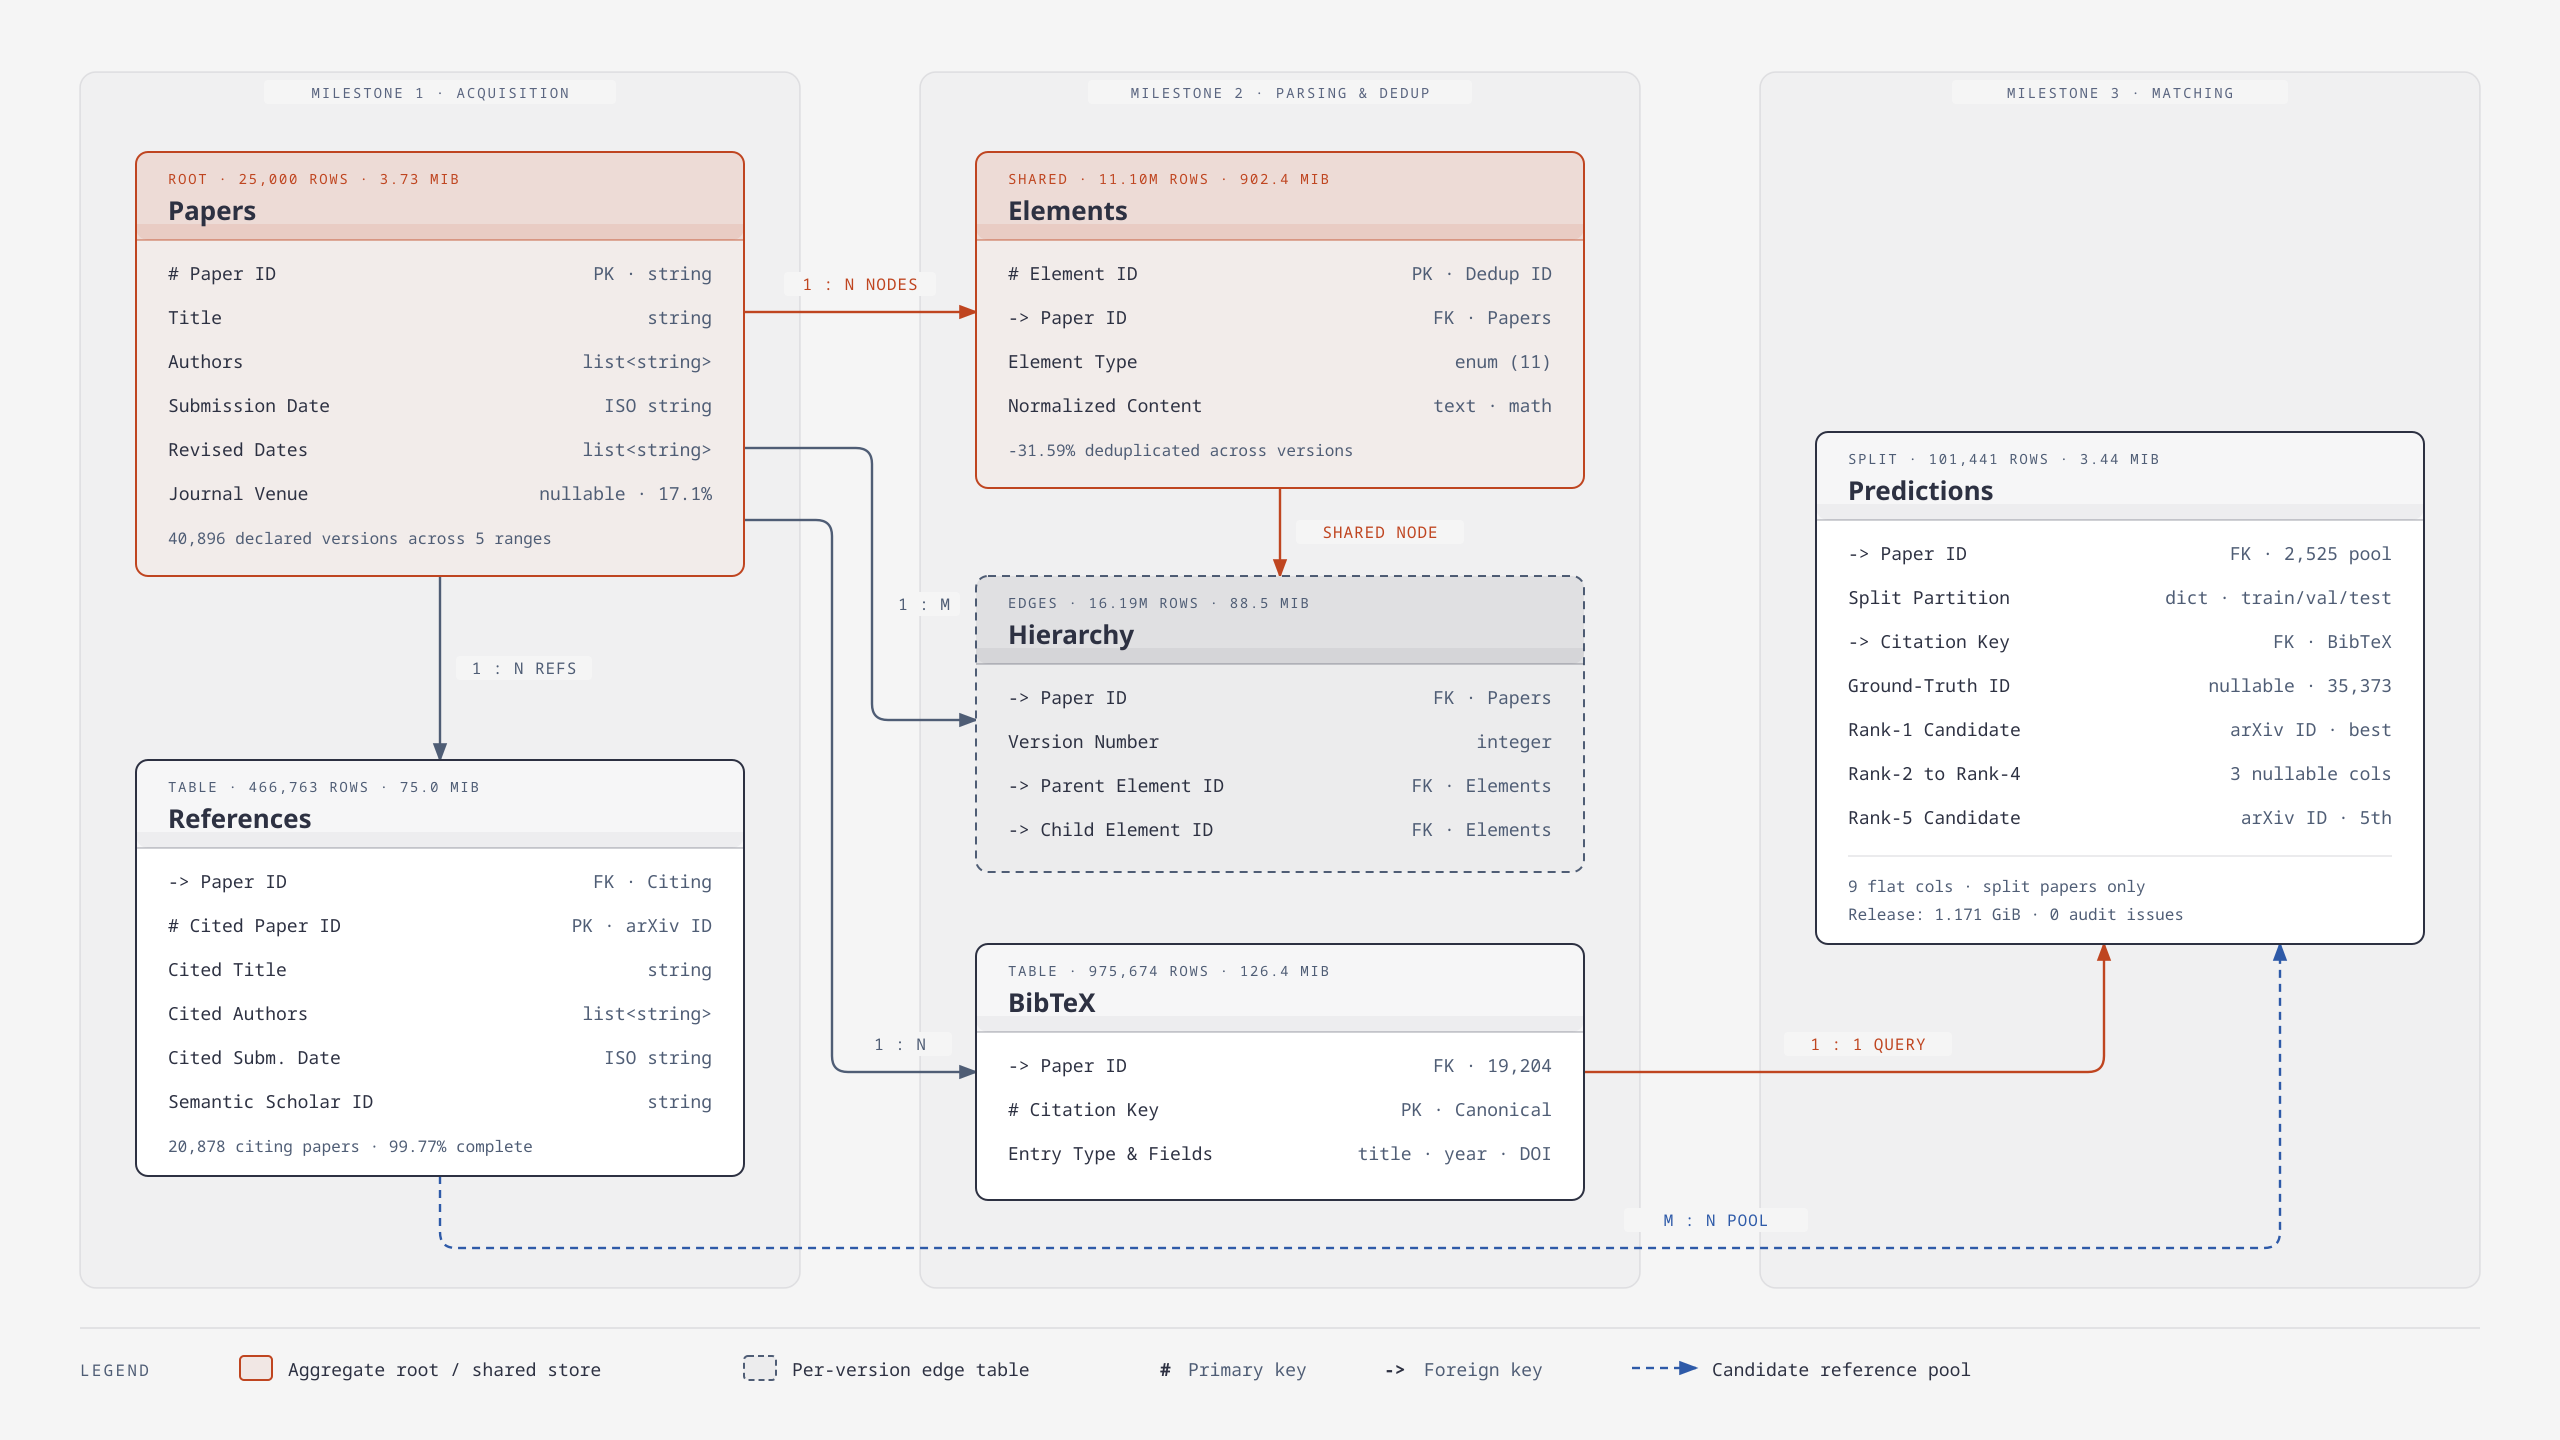
\includegraphics[width=\linewidth]{images/data_schema_er.png}
    \caption[Mô hình thực thể -- liên kết sáu bảng dữ liệu cột Apache Parquet]{Mô hình thực thể -- liên kết chuẩn hóa gồm sáu bảng dữ liệu cột Apache Parquet xoay quanh khóa mã định danh arXiv không phiên bản, tách biệt kho phần tử nội dung đã khử trùng lặp khỏi bảng cạnh quan hệ phân cấp theo từng phiên bản.}
    \label{fig:data_schema_er}
\end{figure}

Cấu trúc quan hệ giữa sáu bảng phát hành được trình bày trực quan tại Hình~\ref{fig:data_schema_er} và đặc tả khái niệm chi tiết trong Bảng~\ref{tab:six_tables}. Toàn bộ lược đồ xoay quanh khóa định danh bài báo arXiv chuẩn hóa không mang hậu tố phiên bản, bảo đảm mọi thực thể từ siêu dữ liệu bài báo, tài liệu tham khảo bên ngoài, cây văn bản đa phiên bản đến kết quả đối sánh đều nối kết nhất quán qua một trục khóa duy nhất. Quyết định chuẩn hóa mang tính nền tảng của mô hình dữ liệu nằm ở việc tách rời bảng phần tử nội dung duy nhất khỏi bảng quan hệ phân cấp theo từng phiên bản: một câu văn hoặc công thức toán học giữ nguyên qua các phiên bản $v_1, v_2, \dots, v_k$ chỉ lưu trữ nguyên văn đúng một lần trong bảng phần tử, trong khi bảng quan hệ phân cấp dùng các bộ khóa nhẹ chỉ mục phiên bản, nút cha và nút con để tái tạo nguyên vẹn cấu trúc cây có thứ tự của từng phiên bản riêng biệt. Tương tự, việc tách biệt bảng mục lục BibTeX khai báo bên trong bài báo với bảng tài liệu tham khảo thu hoạch từ Semantic Scholar giúp phân tách rõ ràng giữa phát biểu trích dẫn của tác giả và tập ứng viên đích ngoài đồ thị tri thức cho đến khi bảng kết quả dự đoán đối sánh liên kết hai phía ở Giai đoạn 3. Trước khi đóng gói phát hành cuối cùng, toàn bộ năm phân mảnh thành viên của cả sáu bảng đều vượt qua quy trình kiểm định tự động về khóa chính, toàn vẹn khóa ngoại và định dạng dữ liệu với kết quả $0$ lỗi phát sinh.

\begin{table}[htbp]
    \centering
    \scriptsize
    \setlength{\tabcolsep}{4pt}
    \renewcommand{\arraystretch}{1.24}
    \begin{tabularx}{\textwidth}{p{0.19\textwidth} c p{0.21\textwidth} X r r}
        \toprule
        \textbf{Bảng dữ liệu} & \textbf{GĐ} & \textbf{Khóa logic \& Quan hệ} & \textbf{Vai trò khái niệm trong kho dữ liệu} & \textbf{Số dòng} & \textbf{Parquet} \\
        \midrule
        Bảng siêu dữ liệu bài báo & GĐ 1 & Khóa chính: mã arXiv không phiên bản (bảng trung tâm $1$) & Lưu tiêu đề, tác giả chuẩn hóa, chuỗi ngày nộp và hiệu chỉnh đầy đủ $v_1 \dots v_N$, nơi công bố chính thức và phạm vi sở hữu. & 25,000 & 3.73 MiB \\
        Bảng tài liệu tham khảo & GĐ 1 & Khóa ghép: mã bài trích dẫn + mã arXiv đích ($1:N$ từ bài báo) & Lưu danh mục bài báo arXiv được trích dẫn thu từ Semantic Scholar kèm tiêu đề, tác giả và ngày nộp $v_1$ chuẩn hóa từ arXiv. & 466,763 & 75.01 MiB \\
        Bảng phần tử nội dung & GĐ 2 & Khóa ghép: mã bài báo + mã phần tử duy nhất ($1:N$ từ bài báo) & Lưu kho văn bản sạch đã khử trùng lặp liên phiên bản cho từng loại nút cấu trúc (mục, câu văn, công thức khối, hình bảng, danh sách). & 11,098,189 & 902.35 MiB \\
        Bảng quan hệ phân cấp & GĐ 2 & Khóa ghép: mã bài báo + phiên bản + nút cha + nút con ($N:M$) & Tái tạo trọn vẹn cây cấu trúc có thứ tự của từng phiên bản bằng cách liên kết các nút thuộc bảng phần tử nội dung. & 16,185,255 & 88.50 MiB \\
        Bảng mục lục BibTeX & GĐ 2 & Khóa ghép: mã bài báo + khóa trích dẫn hợp nhất ($1:N$ từ bài báo) & Hợp nhất các mục thư mục từ nguồn BibTeX và mục tham khảo nội tuyến xuyên phiên bản gồm tiêu đề, tác giả, năm, tạp chí, DOI và liên kết. & 975,674 & 126.41 MiB \\
        Bảng kết quả dự đoán đối sánh & GĐ 3 & Khóa ghép: mã bài báo + khóa trích dẫn mẫu ($1:1$ trên tập mẫu) & Lưu phân hoạch tập dữ liệu, nhãn đối sánh, mã arXiv chuẩn đối chiếu và danh sách năm ứng viên xếp hạng cao nhất của mô hình. & 101,441 & 3.44 MiB \\
        \midrule
        \textbf{Tổng hợp 6 bảng} & \textbf{GĐ 1--3} & \textbf{5 phân mảnh thành viên, 0 lỗi kiểm định toàn vẹn} & \textbf{Kho dữ liệu cột hợp nhất cho toàn bộ $25{,}000$ bài báo chính thức (tương đương $1.171\text{ GiB}$).} & \textbf{28,852,322} & \textbf{1,199.45 MiB} \\
        \bottomrule
    \end{tabularx}
    \caption[Đặc tả khái niệm sáu bảng dữ liệu xuất bản Apache Parquet]{Đặc tả khái niệm sáu bảng dữ liệu chuẩn hóa được xuất bản dưới định dạng lưu trữ cột Apache Parquet cho toàn nhóm ChickenDev. Tổng dung lượng $1{,}199.45\text{ MiB}$ ($1.171\text{ GiB}$) là tổng chính xác trước khi làm tròn hai chữ số thập phân ở từng bảng.}
    \label{tab:six_tables}
\end{table}
